\chapter{Applicazioni Web}
\section{Web statico}
Il web delle origini era un sistema completamente statico:\uline{ il server riceveva la richiesta e si limitava a restituire documenti HTML salvati su disco "cosi' com'erano"}, senza operare alcuna elaborazione dinamica per gli utenti.

Il primo passo per la comunicazione attiva dal client verso il server si è avuto con l'introduzione dei \textbf{form HTML}.
\section{Comunciazione attraverso HTTP}
La comunicazione avviene tramite il protocollo HTTP, che presenta queste caratteristiche chiave:
\begin{itemize}
    \item È un formato basato su testo composto da Header e Body.
    \item Consente di generalizzare la natura dei file in transito utilizzando un identificativo del formato chiamato payload MIME
    \item È "stateless", ovvero non conserva alcuna memoria tra le chiamate: ogni richiesta HTTP è un messaggio autonomo completamente slegato dai precedenti
\end{itemize}

\chapter{Sviluppo lato Client - HTML}
\section{Interazione con il server basate su link}
Il metodo più basilare per l'interazione è l'utilizzo dei link (\texttt{<a>}).

Un link punta a una specifica risorsa remota sul server e, quando viene cliccato, fa in modo che il browser generi ed invii in automatico una \uline{richiesta \texttt{HTTP} di tipo \texttt{GET}} all'URL specificato.

\begin{tcolorbox}{Esempio di link che punta ad una risorsa}
\begin{lstlisting}[language=HTML]
<p>Click the link to ask the servlet to send back an HTML document</p>
<a href="http://localhost:8080/SlideServlet/GetHTTPServlet">
  Get HTML Document
</a>
\end{lstlisting}
\begin{figure}[H]
    \centering
    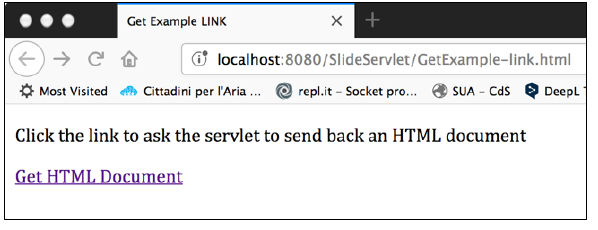
\includegraphics{figures/Schermata_20260512_124943.png}
    \caption{Risultato grafico}
\end{figure}
\end{tcolorbox}

\section{Interazioni basata su form}
I Form (\texttt{<text>}) sono lo strumento \texttt{HTML} dedicato a richiedere e raccogliere input dall'utente per poi inviarlo al server.

A livello di comunicazione HTTP, un form può operare principalmente in due modi:

\subsection{Form con GET}
Se il form utilizza il metodo \texttt{GET}, i valori inseriti dall'utente vengono agganciati direttamente all'URL della richiesta sotto forma di \texttt{Query parameter}
\begin{tcolorbox}{Esempio di form con metodo GET}
\begin{lstlisting}[language=HTML]
<form action="http://localhost:8080/SlideServlet/GetHTTPServlet" method="GET">
    <p>Click the button to have the servlet send an HTML document</p>
    <input type="submit" value="Get HTML Document">
</form>
\end{lstlisting}
\begin{figure}[H]
    \centering
    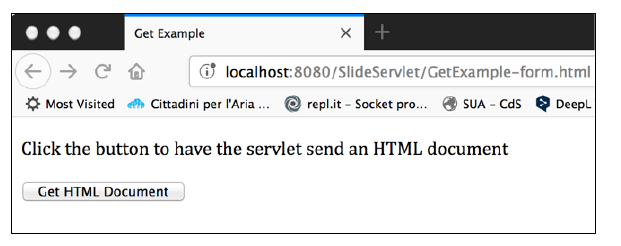
\includegraphics[scale=0.5]{figures/Schermata_20260512_150719.png}
    \caption{Risultato grafico}
\end{figure}
\end{tcolorbox}

\subsection{Form con POST}
Se il form utilizza il metodo \texttt{POST}, i dati vengono invece incapsulati in modo più nascosto all'interno del payload (il corpo centrale del messaggi \texttt{HTTP}), mantenendo l'URL pulito.
\begin{tcolorbox}{Esempio di form con metodo POST}
\begin{lstlisting}[language=HTML]
<form action="http://localhost:8080/SlideServlet/PostHTTPServlet" method="POST">
What is your favorite pet?<br> <br>
<input type="radio" name="animal" value="dog">Dog<br>
<input type="radio" name="animal" value="cat">Cat<br>
<input type="radio" name="animal" value="bird">Bird<br>
<input type="radio" name="animal" value="snake">Snake<br>
<input type="radio" name="animal" value="none" checked>None<br>
<br> <input type="submit" value="Submit"> <input type="reset">
</form>
\end{lstlisting}
\begin{figure}[H]
    \centering
    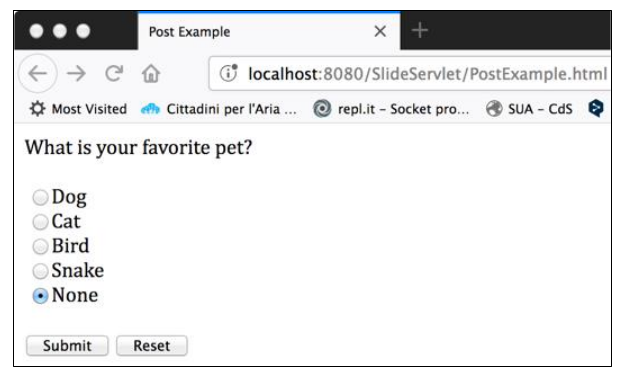
\includegraphics[scale=0.5]{figures/Schermata_20260512_151336.png}
    \caption{Risultato grafico}
\end{figure}
\end{tcolorbox}

\subsection{Limiti dei Form}
I form \texttt{HTML} nativi possiedono un limite importante: supportano solamente 3 tipi di codifica standard (i cosiddetti enctype) e \uline{non contemplano l'uso nativo di formati strutturati come JSON o XML}

\chapter{Sviluppo lato Server - Servlet Java}
\section{Definizione}
Le servlet sono piccole applicazioni e oggetti scritti in Java che vivono all'interno della memoria di un server.

Non funzionanon in modo autonomo, ma vengono gestite da un ambiente di esecuzione detto Servlet Container (o application server, come Apache Tomcat), il quale si fa carico di accenderle, segnerle e inoltrare loro il traffico di rete.

\section{Configurazione di una servlet}
Le servlet richiedono una configurazione che definisca:
\begin{itemize}
    \item Nome della servlet
    \item Classe di implementazione
    \item Mapping URL
    \item Parametri di inizializzazione
\end{itemize}

\section{Metodi}
\subsection{Metodi del ciclo di vita}
A livello di codice, ogni Servlet implementa l'interfaccia \texttt{jakarta.servlet.Servlet} che possiede come metodi:
\begin{itemize}
    \item \texttt{void init(ServletConfig config)}

    Inizializza la servelet, viene invocata dopo la creazione della stessa.

    \begin{tcolorbox}[title={Esempio di metodo init}, breakable]
        \begin{lstlisting}[language=java]
@WebServlet(
    urlPatterns = "/LaMiaServlet",
    initParams = { 
        @WebInitParam(name = "emailAmministratore", value = "admin@miosito.it") 
    }
)
public class MiaServlet extends HttpServlet {

    private String emailDiContatto;

    @Override
    public void init(ServletConfig config) throws ServletException {
        super.init(config);

        // E' buona norma richiamare il metodo della superclasse
        emailDiContatto = config.getInitParameter("emailAmministratore");
        
        System.out.println("Servlet caricata. Email impostata a: " + emailDiContatto);
    }

    @Override
    protected void doGet(HttpServletRequest request, HttpServletResponse response) {
        // Qui la Servlet puo' usare la variabile emailDiContatto
    }
}
        \end{lstlisting}
    \end{tcolorbox}
    \item \texttt{void destroy()}

    Chiamata quando la servlet termina (es: per chiudere un file o una connessione con un database)
    \begin{tcolorbox}[title={Esempio del metodo destroy}, breakable]
        \begin{lstlisting}[language=java]
public class ShutdownServlet extends HttpServlet {

    // 1. Inizializzazione
    @Override
    public void init() throws ServletException {
        System.out.println("Servlet avviata e pronta.");
    }

    // 2. Servizio (Eseguito ad ogni richiesta)
    @Override
    protected void doGet(HttpServletRequest req, HttpServletResponse res) 
            throws IOException {
        res.getWriter().println("Servlet in esecuzione...");
    }

    // 3. Distruzione (Eseguito una sola volta alla chiusura)
    @Override
    public void destroy() {
        // Qui si chiudono connessioni al DB o file aperti
        System.out.println("Salvataggio dati in corso... Servlet rimossa.");
    }
}
        \end{lstlisting}
    \end{tcolorbox}
    \item \texttt{void service(ServletRequest request, ServletResponse response)}

    \begin{tcolorbox}[title={Esempio del metodo service}, breakable]
\begin{lstlisting}[language=java]
public class MiaServletService extends HttpServlet {

    /**
     * Il metodo service() intercetta ogni richiesta.
     * Nota: usa ServletRequest e ServletResponse (generici).
     */
    @Override
    public void service(ServletRequest request, ServletResponse response) 
            throws ServletException, IOException {
        
        response.setContentType("text/html");
        
        // Questo messaggio apparira' sia per richieste GET che POST
        response.getWriter().println("<html><body>");
        response.getWriter().println("<h1>Richiesta intercettata dal metodo service!</h1>");
        response.getWriter().println("<p>Gestione universale senza distinzione tra i verbi HTTP.</p>");
        response.getWriter().println("</body></html>");
    }
}
\end{lstlisting}
\end{tcolorbox}

    Invocato per getire le richieste del client
    \item \texttt{ServletConfig getServletConfig()}

    Restituisce i parametri di inizializzazione e il \textsl{ServletContext} che da accesso all'ambiente.
    \item \texttt{String getServletInfo()}

    Restituisce informazioni tipo autore e versione
\end{itemize}
\subsection{Metodi classe \texttt{HTTPServlet}}
Nella pratica comune, si estende la classe \texttt{HttpServlet}.

Questa classe fornisce metodi specifici per gestire i diversi verbi del protocollo HTTP.
\begin{itemize}
    \item \texttt{doGet(HttpServletRequest req, HttpServletResponse res)}

    Gestisce le richieste di tipo \texttt{GET}.

    È usato tipicamente per recuperare informazioni dal server senza modificarne lo stato

    \begin{tcolorbox}[breakable, title={Esempio del metodo GET}]
        \begin{lstlisting}
public class SalutoServlet extends HttpServlet {

    // Gestisce le richieste di lettura (GET)
    @Override
    protected void doGet(HttpServletRequest request, HttpServletResponse response) 
            throws ServletException, IOException {
        
        // Prepariamo la risposta per il browser
        response.setContentType("text/html");
        PrintWriter out = response.getWriter();

        // Inviamo il contenuto HTML
        out.println("<html><body>");
        out.println("<h1>Ciao!</h1>");
        out.println("<p>Questa e' una risposta generata dal metodo doGet.</p>");
        out.println("</body></html>");
    }
}
        \end{lstlisting}
    \end{tcolorbox}
    \item \texttt{doPost(HttpServletRequest req, HttpServletResponse res)}

    Gestisce le richieste \texttt{POST}.
    \item \texttt{doPut() / doDelete()}
\end{itemize}
\subsection{Metodi per gestire Richieste (\texttt{HttpServletRequest})}
Questi metodi permettono di accedere ai dati contenuti nell'header e nel body del messaggio \texttt{HTTP} inviato dal client:
\begin{itemize}
    \item \texttt{getParameter(String name)}

    Restituisce il valore associato al parametro specificato, tipicamente proveniente da una query string o da un form \texttt{HTML}
    \item \texttt{getParameterNames()}

    Restituisce un'enumerazione contenente l'elenco di tutti i nomi dei parametri passati nella richiesta.
    \item \texttt{getParametersValues(String name)}

    Restituisce un array di stringhe contenente tutti i valori associati a un determinato parametro.
    \item \texttt{getCookies()}

    Restituisce un array contenente tutti i cookie memorizzati sul client e inviati al server con la richiesta.
    \item \texttt{getSession(boolean create)}

    Restituisce l'oggetto \texttt{HTTPSession} che identifica l'utente corrente per la gestione dello stato.

    Se \texttt{create} è impostato a \texttt{true}, crea una nuova sessione qualora non ne esista già una.
\end{itemize}
\subsection{Metodi per gestire le Risposte (\texttt{HttpServletResponse})}
Questi metodi permettono di configurare la risposta \texttt{HTTP} da inviare al client, impostando header, status code e il contenuto del body:
\begin{itemize}
    \item \texttt{setContentType(String type)}

    Specifica il tipo MIME del contenuto della risposta, in modo da comunicare al browser come deve interpretare e visualizzare i dati ricevuti.
    \item \texttt{getWriter()}

    Restituisce uno stream di caratteri (oggetto \texttt{PrintWriter}) utilizzato per scrivere testo all'interno del corpo della risposta.
    \item \texttt{getOutputStream()}

    Restituisce uno stream di byte (\texttt{ServletOutputStream}) utilizzato per scrivere dati binari nel corpo della risposta.
    \item \texttt{addCookie(Cookie cookie)}

    Aggiunge un nuovo cookie all'interno dell'intestazione (header) della risposta, in modo che il browser del client lo memorizzi localmente.
\end{itemize}
\section{MultiThreadding - Modello a Thread Pool e l'esecuzione}
Il multithreadding nella Servlet Java si basa su un'architettura fondamentale: \uline{molti thread attraversona una singola istanza della servlet}.

A differenza di tecnologie storiche che creavano un processo separato per ogni utente, le servlet sono progettate per massimizzare la scalabilità.

Le servlet sono oggetti Java che risiedono nella memoria del server, ma non avviano thread per conto proprio: il codice dei loro metodi viene eseguito da thread creati e gestiti direttamente dal container.

Per ottimizzare i tempi di risposta, il container utilizza il pattern architetturale del \textbf{Thread pool}.

Questo significa che:
\begin{enumerate}
    \item Vie pre-creato un gruppo fisso di thread che rimangono in attesa di lavoro.
    \item Quando arriva una richiesta \texttt{HTTP} da un client, il container non istanza una nuova servlet e non crea un nuovo thread da zero, ma preleva un thread dal pool e gli fa eseguire il metodo \texttt{doX} sulla singola istanza condivisa della servlet.
    \item La dimensione del pool fissa un limite massimo al numero di threadche possono esistere contemporaneamente.
\end{enumerate}

\subsection{Vantaggi}
Questa scelta progettuale ha diverse motivazioni che migliorano nettamente le prestazioni del server:
\begin{itemize}
    \item \textbf{Risparmio di memoria}: Esistendo una sola istanza dell'oggetto servlet per tutti i client, si consuma una quantità di memoria minima.
    \item \textbf{Velocità}: Si abbattono i costi e i tempi legati all'inizializzazione ripetuta degli oggetti e alla creazione "on the fly" dei thread.
    \item \textbf{Persistenza}: Abilita la possibilità di mantenere in memoria risorse costose e condividerle tra varie richieste, come ad esempio un pool di connesioni a un database.
\end{itemize}

\chapter{Sviluppo lato Server - Java Server Pages}
\section{Definizione}
Le JSP (Java Server Pages) sono una tecnologia nata per facilitare la creazione di interfacce web dinamiche, separando la parte statica della pagina dalla logica applicativa.

La caratteristica più affascinante delle JSP è che \uline{non vengono interpretate direttamente}.

Quando un client richiede una pagina JSP per la prima, il server la traduce automaticamente in codice Java, la compila in un file \texttt{.class}(bytecode) e la esegue come se fosse una normalissima Servlet.

\section{Elementi di una pagina JSP}
All'interno di un JSP si mescola in normale testo \texttt{HTML} con elementi specifici racchiusi in particolari tag.

Questi elementi si dividono in 3 categorie principali:
\begin{itemize}
    \item \textbf{Direttive (\texttt{<\% @ \%>})}

    Danno istruzioni generali al server su come compilare la pagina.
    \begin{tcolorbox}[title={Esempio JSP: Direttiva page}, breakable]
        \begin{lstlisting}[language=html]
<%-- Direttiva page: imposta il tipo di contenuto e importa una classe --%>
<%@ page language="java" contentType="text/html; charset=UTF-8" import="java.util.Date" %>

<html>
    <body>
        <h1>Esempio Direttiva JSP</h1>
        <p>
            <%-- Usiamo la classe Date importata sopra --%>
            La data e l'ora attuale sono: <%= new Date() %>
        </p>
    </body>
</html>
        \end{lstlisting}
    \end{tcolorbox}
    \item \textbf{Azioni (\texttt{<jsp:XXX>})}

    Vengono processate a ogni singola richiesta e permettono di eseguire operazioni complesse senza scrivere codice Java puro:
\begin{tcolorbox}[title={Esempio di Azioni JSP}, breakable]
\begin{lstlisting}[language=html]
<html>
<body>
    <h1>Pagina Principale</h1>

    <%-- 1. Azione include: include il file al momento della richiesta --%>
    <jsp:include page="data_corrente.jsp" />

    <p>Il contenuto sopra e' stato incluso dinamicamente.</p>

    <%-- 2. Esempio di forward (commentato per non bloccare la pagina)
         Questa azione interrompe la pagina attuale e manda l'utente altrove.
    <jsp:forward page="login.jsp" /> 
    --%>
</body>
</html>
\end{lstlisting}
\end{tcolorbox}
    \item \textbf{Elementi di Scripting}

    Permettono di inserire frammenti di codice Java vero e proprio.

    Si dividono in: 
    \begin{itemize}
        \item \textbf{Scriptlet (\texttt{<\% \%>})} per istruzioni e cicli.
        \item \textbf{Declaration \texttt{<\%! \%>}} per dichiarare variabili o metodi.
        \item \textbf{Expression \texttt{<\%= \%>}} per valutare un espressione e stamparne direttamente il risultato nell'\texttt{HTML.}
    \end{itemize}
\begin{tcolorbox}[title={Esempio costrutti JSP}, breakable]
\begin{lstlisting}[language=html]
<%@ page language="java" contentType="text/html; charset=UTF-8" %>
<html>
<body>
    <%! 
        // 1. DECLARATION (<%! %>): Dichiariamo una variabile e un metodo
        private String titolo = "Lista Numerica";
        
        public String trasformaInMaiuscolo(String testo) {
            return testo.toUpperCase();
        }
    %>

    <h1><%= trasformaInMaiuscolo(titolo) %></h1> 
    <%-- 2. EXPRESSION (<%= %>): Valuta e stampa il titolo in maiuscolo --%>

    <ul>
    <% 
        // 3. SCRIPTLET (<% %>): Usiamo un ciclo for per la logica
        for(int i = 1; i <= 3; i++) {
    %>
        <li>Iterazione numero: <%= i %></li> 
        <%-- Un'altra EXPRESSION per stampare l'indice del ciclo --%>
    <% 
        } // Chiusura dello scriptlet del ciclo
    %>
    </ul>
</body>
</html>
\end{lstlisting}
\end{tcolorbox}
\end{itemize}

\section{Esempio}

\begin{tcolorbox}[
    title={Esempio JSP e Anteprima},
    sidebyside,                 % Attiva l'affiancamento
    lefthand width=0.6\textwidth, % La parte sinistra occupa il 60%
    % NOTA: Abbiamo rimosso 'breakable' per permettere il sidebyside
]

% --- PARTE SINISTRA: Il codice ---
\begin{lstlisting}[language=html, frame=none]
<%@ page language="java" contentType="text/html; charset=UTF-8" %>
<!DOCTYPE html>
<html>
<body>
    <h1>Esempio JSP Compatto</h1>
    <%
        String nome = "Utente";
        int numero = 5;
    %>
    <p>Ciao, <%= nome %>!</p>
</body>
</html>
\end{lstlisting}

\tcblower % --- SEPARATORE: Tutto cio' che segue va a DESTRA ---

% --- PARTE DESTRA: L'immagine ---
\centering
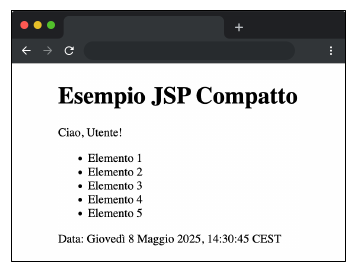
\includegraphics[width=\linewidth]{figures/Schermata_20260512_173654.png}
\end{tcolorbox}

\section{Oggetti impliciti}
Per facilitare la scrittura del codice, l'ambiente JSP mette automaticamente a disposizione dello sviluppatore 9 oggetti impliciti senza che ci sia bisogno di istanziarli automaticamente.

\begin{itemize}
    \item \texttt{request}: Rappresenta la richiesta HTTP inviata dal client. 
    
    Si usa per recuperare parametri del form, header e informazioni sul browser dell'utente.
    \item \texttt{response}: Rappresenta la risposta HTTP inviata al client. 
    
    Serve per impostare header, aggiungere cookie o effettuare reindirizzamenti (redirect).
    \item \texttt{out}: È l'oggetto (JspWriter) utilizzato per scrivere il contenuto nel corpo della risposta che verrà inviata al browser.
    \item \texttt{page}: Rappresenta l'istanza corrente della Servlet generata dalla pagina JSP (equivale al \texttt{this} in Java).
    \item \texttt{pageContext}: Fornisce l'accesso a tutti i contesti della pagina e permette di gestire gli attributi in vari ambiti (scope).
    \item \texttt{session}: Rappresenta la sessione dell'utente. 
    
    Permette di memorizzare informazioni che devono persistere mentre l'utente naviga tra diverse pagine del sito.
    \item \texttt{application}: Rappresenta l'intera applicazione web (ServletContext). 
    
    I dati salvati qui sono condivisi da tutti gli utenti e da tutte le pagine.
    \item \texttt{config}: Rappresenta la configurazione della Servlet (ServletConfig) e permette di leggere eventuali parametri di inizializzazione definiti nel file \texttt{web.xml}.
    \item \texttt{exception}: Disponibile solo se la pagina è definita come "pagina di errore". 
    
    Contiene l'eccezione che ha causato il malfunzionamento.
\end{itemize}

\subsection{Scope (visibilità)}
Ognuno di questi oggetti, cosi' come qualsiasi variabile create nell'applicazione, possiede uno "scope" (ambito).

Lo scope è fondamentale perchè \uline{determina il ciclo di vita e il livello di visibilità} dell'oggetto nella memoria del server.

Esistono 4 livelli di scope:
\begin{itemize}
    \item \textbf{Page}: È il livello base.

    L'oggetto esiste ed è visibile solo all'interno della specifica pagina JSP che lo ha creato.
    \item \textbf{Request}: L'oggetto vive per il tempo necessario a elaborare una singola richiesta \texttt{HTTP}.

    È utile se la richiesta viene passata tra più componenti.
    \item \textbf{Session}: L'oggetto è legato alla sessione del singolo utente.

    I dati salvati qui rimangono in memoria e sono condivisi tra tutte le pagine visitate da quell'utente specifico.
    \item \textbf{Application}: È il livello massimo.

    L'oggetto è condiviso in modo globale tra tutti gli utenti e tutte le pagine dell'intera applicazione web.
\end{itemize}

\section{JavaBean}
L'uso eccessivo di Scriptlet rende le pagine JSP caotiche e impossibili da manutenere per i web designer, per risolvere questo problema si utilizzano i JavaBean.

Un JavaBean è una semplicissima classe Java (POJO) che funge da contenitore di dati e logica, e deve rispettare regole rigide: 
\begin{itemize}
    \item deve essere pubblica
    \item deve avere costruttore senza argomenti
    \item deve avere attributi priva e metodi pubblici get e set per accedere a quegli attributi
\end{itemize}

Invece di scrivere codice Java complesso, la JSP utilizza delle speciali "Azioni" per interagire con il Bean in modo pulito:

\begin{itemize}
    \item \textbf{\texttt{<jsp:useBean>}}: Cerca un Bean in un determinato scope o lo istanzia se non esiste.
    \item \textbf{\texttt{<jsp:getProperty>} e \texttt{<jsp:setProperty>}}: Leggono o scrivono le proprietà del Bean.
    
    Un aspetto molto potente è l'uso di \texttt{property="*"}.
    
    Quando viene usata, il server legge in automatico tutti i parametri in arrivo da un form HTML e invoca i rispettivi metodi set del Bean convertendo i tipi di dato, eliminando completamente la necessità di leggere e convertire manualmente i dati della richiesta.
\end{itemize}

\section{Declino}
Nonostante i tentativi di incapsulare la logica (come i JavaBean e il pattern MVC), il modello basato su JSP è considerato oggi superato a causa di intrinsechi \textbf{limiti architetturali} \textsuperscript{19}.

I motivi principali del suo declino sono:

\begin{itemize}
    \item \textbf{Forte accoppiamento (Spaghetti Code):} 
    L'inserimento di frammenti Java (scriptlet) dentro l'HTML rende il codice molto difficile da leggere, testare e manutenere \textsuperscript{19}.
    \item \textbf{Sviluppo lento:} Poiché le JSP devono essere tradotte in Servlet e compilate dal server, il ciclo di sviluppo e testing risulta molto più lento rispetto a tecnologie moderne \textsuperscript{19}.
    \item \textbf{Evoluzione del Web:} Le JSP sono nate nel 1999 per generare pagine interamente sul server \textsuperscript{20}. Oggi, il paradigma dominante si è spostato verso le \textbf{Single Page Application (SPA come React, Angular, Vue)}, dove il browser si occupa di costruire la View dinamicamente (client-side), mentre il server funge solo da fornitore di dati puri (JSON) tramite \textbf{servizi REST} \textsuperscript{20}.
    \item \textbf{Alternative Server-Side:} Anche quando serve generare l'HTML sul server, oggi si preferiscono \textbf{motori di template moderni come Thymeleaf}, che garantiscono una separazione molto più rigida tra il codice HTML e la logica Java, oppure framework per il Server-Side Rendering ibrido (come Next.js o Nuxt) \textsuperscript{20}.
\end{itemize}